% background.tex - Contextual capabilities

\section{Contextual Capabilities}
\label{sec:background}

The easiest way to understand contextual capabilities is to start from a
mechanism every reader already knows: ordinary function parameters. %
If an operation needs an output channel, a logger, and a user-scoped orders
service, one direct design is to pass all of them explicitly:
\[
\texttt{handle(req, out, logger, orders)}
\]
and then continue threading those same parameters through helpers that may not
use them directly:
\[
\begin{array}{l}
\texttt{handle(req, out, logger, orders)} \\
\rightarrow\ \texttt{plan(task, out, logger, orders)} \\
\rightarrow\ \texttt{respond(plan, out, logger, orders)}
\end{array}
\]
This style is explicit and testable, but it is also noisy. %
Intermediate functions often carry capabilities only so later code can
eventually use them. %

Contextual capabilities keep the good part of parameter passing and remove that
plumbing cost. %
A capability is still an ordinary typed value, but it may be \emph{bound for a
  context} rather than passed through every signature. %
Code deeper in the call chain can then use that capability because the
surrounding context makes it available. %
In that sense, capabilities behave like remotely bound parameters that propagate
through the call chain automatically, while remaining statically tracked and
explicitly controllable. %

\begin{figure}[t]
\centering
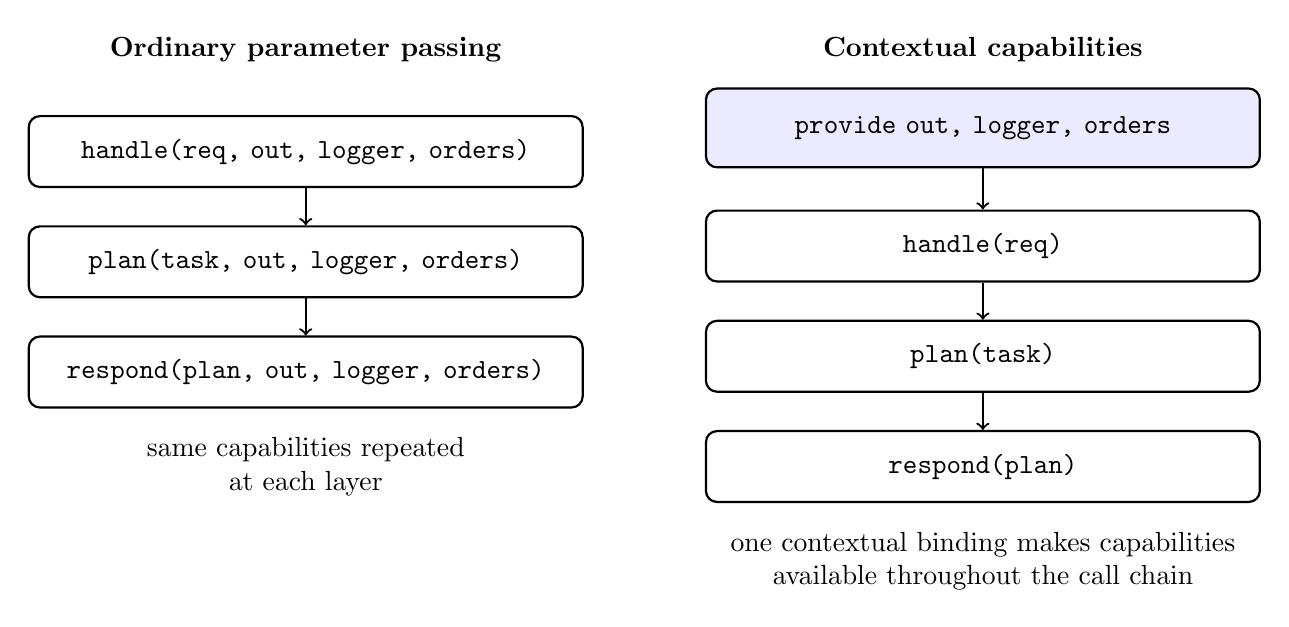
\begin{tikzpicture}[
  fn/.style={draw, rounded corners, thick, align=center, text width=6.8cm, minimum height=0.9cm},
  ctx/.style={draw, rounded corners, fill=blue!8, thick, align=center, text width=6.8cm, minimum height=1.0cm},
  note/.style={align=center}
]
  \node[note] at (-4.3,2.2) {\textbf{Ordinary parameter passing}};
  \node[fn] (h1) at (-4.3,0.9) {\texttt{handle(req, out, logger, orders)}};
  \node[fn] (p1) at (-4.3,-0.5) {\texttt{plan(task, out, logger, orders)}};
  \node[fn] (r1) at (-4.3,-1.9) {\texttt{respond(plan, out, logger, orders)}};
  \draw[->, thick] (h1) -- (p1);
  \draw[->, thick] (p1) -- (r1);
  \node[note] at (-4.3,-3.1) {same capabilities repeated\\at each layer};

  \node[note] at (4.3,2.2) {\textbf{Contextual capabilities}};
  \node[ctx] (c) at (4.3,1.2) {\texttt{provide out, logger, orders}};
  \node[fn] (h2) at (4.3,-0.3) {\texttt{handle(req)}};
  \node[fn] (p2) at (4.3,-1.7) {\texttt{plan(task)}};
  \node[fn] (r2) at (4.3,-3.1) {\texttt{respond(plan)}};
  \draw[->, thick] (c) -- (h2);
  \draw[->, thick] (h2) -- (p2);
  \draw[->, thick] (p2) -- (r2);
  \node[note] at (4.3,-4.3) {one contextual binding makes capabilities\\available throughout the call chain};
\end{tikzpicture}
\caption{Ordinary parameter plumbing versus contextual capability propagation}
\label{fig:contextual-propagation}
\end{figure}

\autoref{fig:contextual-propagation} is the central intuition. %
Contextual capabilities do not make authority ambient. %
They make authority available through explicit program context. %
A caller may bind an output capability for a single execution. %
Trusted code may rebind a user-scoped orders capability for one region of
computation. %
A closure may package a capability behind a narrower interface. %
In each case, the capability remains an ordinary value; what changes is only how
it becomes available to the code that uses it. %

\paragraph{The Challenge.}
The challenge is to give this convenience a sound static account. %
A capability should be usable only when some program context has explicitly
provided it, even in the presence of deep and complex transitive call chains and
first-class functions. %

Lambdas make that harder. %
A closure may carry capability usage transitively: it may use a capability
itself, or call another function that uses it. %
A formal model therefore has to track not only direct capability access, but
also capability use delayed through closure capture and later invocation. %

The calculus \lambdaCC{} provides a formal foundation for statically checked
contextual capabilities. %
